\section{Introduction}
\label{introductionsection}
The use of unmanned aerial vehicles (UAVs) or drones is rising rapidly nowadays. The first documented use of a drone for warfare occurred in  1849 when an unmanned balloon loaded with explosives attacked another town~\cite{mckenna2016public}. After that, a generation of drones is sparked in 1903 by the development of the fixed-wing aircraft. The US army improved drones as weapons during the First World War, but those innovative drones were not deployed before the war ended in 1918. The first use of the drone in the military was in World War II as a surveillance aircraft. After World War II, the Cold war between many countries increased, enhancing the use of drones. Many armed forces started using drones as a weapon, a reconnaissance tool, and a decoy. The progress of drone inspired both military and non-military companies to invest more in the field of drone research and development.

The drone developed exponentially for surveillance of the region or supervision of remote construction projects. The rapid advances in sensing, battery, and aeronautics technology, together along with autonomous navigation methods and low-cost digital cameras have helped make the drone more powerful, safer, and easier to operate \cite{liu2014review}. Since the early pioneering days, almost all types of active and passive sensors have been mounted on aerial systems, ranging from tethered to autonomous or manually operated \cite{sensing2015disasters, dong2013comprehensive}. With the help of these sensors, a drone can be deployed in many sectors, such as building inspection, rescue missions, following an unidentified person, etc. In the present day, large numbers of organizations in different sectors are using drones to visually monitor the problems, find solutions, and even solve the problem based on the task. Such systems are aimed at achieving more efficient service, inspection, and maintenance with minimal human intervention.

The drone-based technique allows low-cost and frequent inspections, high-resolution image analysis and limited human interference, allowing for predictive maintenance at reduced costs~\cite{morgenthal2014quality}. Lots of real-time problems exhibit recognizable visual characteristics that drones can portray with RGB cameras~\cite{roy2013performance}. For example, cracks in the concrete of other surfaces are visible by naked eyes. But it takes substantial manual effort to obtain damage information from a scale area. Additionally, manual inspection is not only challenging but also risky in some cases. Taking pictures at a height from 40 to 50 feet is dangerous because it may be lethal if someone falls from that altitude. Besides, important information might be left behind. But in serval cases, regular monitoring is necessary which can prevent several accidents, e.g., windmill turbine monitoring, building crack inspection, long bridge health investigation. By supplying experts with automated feedback on highly likely locations of destruction, we can significantly reduce the required man-hours and simultaneously increase the efficiency of manual detection, while reducing the human costs associated with the data inspection. Besides building inspection, drones can be used for human suspectable activity monitoring or rule-breaking vehicle tracking~\cite{ngo2019isir}. Drones with other sensors can represent other information, that can improve our daily livings in many ways~\cite{roy2015aarpa, pathak2015acoustic}. Insulation issues in built-up environments can be detected using a drone thermal camera which can save energy~\cite{khan2019detecting, khan2015demo, khan2020temporal}. Common applications of drones in different sectors are shown in Fig~\ref{applicaitonfig}.

\begin{figure}[h!]
\centering
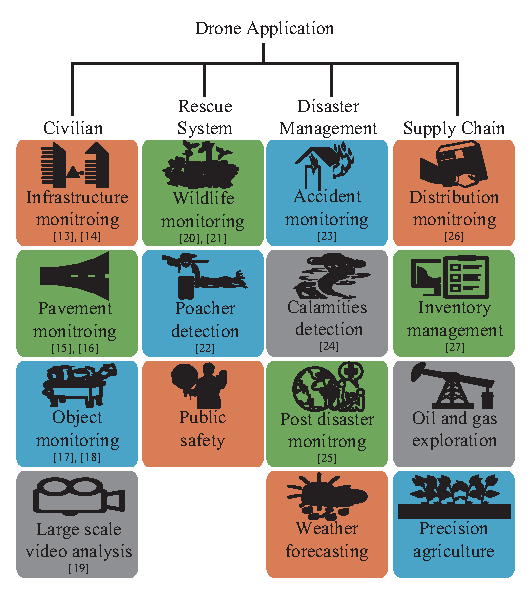
\includegraphics[width=\linewidth]{figure/applicaitonfig.eps}
\caption{Application of drone in different sector.}
\label{applicaitonfig}
\end{figure}
%\begin{table}[h]
\centering
\caption{Application of drones in different sector}
\begin{tabular}{|l|l|}
\hline
Category                             & \multicolumn{1}{c|}{Application}                                                                                             \\ \hline
\multirow{4}{*}{Civilian}            & Infrastructure crack detection~\cite{kucuksubasi2018transfer, kang2018autonomous}                                            \\ \cline{2-2} 
                                     & Road or pavement monitoring~\cite{wu2018coupling, fan2019real}                                                               \\ \cline{2-2} 
                                     & Object detection~\cite{li2017visual,saribas2019hybrid}                                                                       \\ \cline{2-2} 
                                     & Large scale video analysis~\cite{zhang2019dense}                                                                             \\ \hline
\multirow{2}{*}{Rescue system}       & Wildlife monitoring~\cite{mayer2019drones,brennan2019drones}                                                                 \\ \cline{2-2} 
                                     & Poacher detector~\cite{bondi2018spot}                                                                                        \\ \hline
\multirow{3}{*}{Disaster management} & \begin{tabular}[c]{@{}l@{}}Autonomous system able to explain\\ accident situations~\cite{garcia2018explainable}\end{tabular} \\ \cline{2-2} 
                                     & \begin{tabular}[c]{@{}l@{}}Calamities detector such as wildfire\\ with cameras~\cite{kyrkou2019deep}\end{tabular}            \\ \cline{2-2} 
                                     & Post-disaster assessment~\cite{tariq2018dronaid}                                                                             \\ \hline
\multirow{2}{*}{Supply Chain}        & \begin{tabular}[c]{@{}l@{}}Production and distribution monitoring\\ and prediction~\cite{apolo2020deep}\end{tabular}         \\ \cline{2-2} 
                                     & Inventory management~\cite{fernandez2019towards}                                                                             \\ \hline
\end{tabular}
\label{droneapplication}
\end{table}



\begin{comment}
% Please add the following required packages to your document preamble:
% \usepackage{multirow}
\begin{table}[]
\begin{tabular}{|l|l|}
\hline
Category                                                                    & Application                    \\ \hline
\multirow{4}{*}{Military}                                                   & Surveillance                   \\ \cline{2-2} 
                                                                            & Security                       \\ \cline{2-2} 
                                                                            & Air strike                     \\ \cline{2-2} 
                                                                            & Enemy tracking                 \\ \hline
\multirow{8}{*}{Commercial}                                                 & Shipping                       \\ \cline{2-2} 
                                                                            & Filming                        \\ \cline{2-2} 
                                                                            & Crop monitroing                \\ \cline{2-2} 
                                                                            & Irrigation                     \\ \cline{2-2} 
                                                                            & Architecture safety inspection \\ \cline{2-2} 
                                                                            & Mapping                        \\ \cline{2-2} 
                                                                            & Weather forecasting            \\ \cline{2-2} 
                                                                            & Supply chain                   \\ \hline
\multirow{5}{*}{\begin{tabular}[c]{@{}l@{}}Non-profit\\ usage\end{tabular}} & Traffic monitoring             \\ \cline{2-2} 
                                                                            & Rescue operation               \\ \cline{2-2} 
                                                                            & Disaster management            \\ \cline{2-2} 
                                                                            & Photography                    \\ \cline{2-2} 
                                                                            & Human health                   \\ \hline
\end{tabular}
\end{table}
\end{comment}

Though drones have a lot of useful applications, several challenges need to overcome, starting from the navigation system to maintaining the privacy of people. Therefore, in this paper, we have discussed various applications of drones. Besides, we have presented several challenges, including laws and legislation of different countries regarding drones. We also have mentioned the contribution of drones regarding tackling pandemics like COVID19. The organization of the paper is given below.

\subsection*{\textbf{Overview}}
In this article, we briefly discussed drone application in different section, such as, package delivery, site monitoring, disaster management, oil-gas exploration, weather forecasting, wildlife monitoring, precision agriculture~\cite{kucuksubasi2018transfer, kang2018autonomous, wu2018coupling, fan2019real, li2017visual,saribas2019hybrid, zhang2019dense, mayer2019drones,brennan2019drones, bondi2018spot,garcia2018explainable, kyrkou2019deep, tariq2018dronaid, apolo2020deep, fernandez2019towards}.  Section~\ref{introductionsection} presents a short introduction, including a brief history of the drone's invention and evaluation story. Section~\ref{networkingsection} is divided into two subsections. In the following three subsections, we have discussed a few frameworks for autonomous drone navigation, how we can make the operation safer with obstacle avoidance technique, and we can handle drone data more efficiently. 
%In section~\ref{signalprocessingsection}, we have introduced research works that are aimed to handle drone data more efficiently. 
In section~\ref{applicationsection}, we have mentioned machine learning-based drone applications that can improve our daily life. In section~\ref{datasetsection}, we have provided some datasets that are prepared by drones. In section~\ref{toolkitsection}, we have analyzed the hardware part of a drone. In section~\ref{covid19section}, we have described the impact of COVID-19 on drone usage and drone sale. In section~\ref{challengesection}, we have depicted the upcoming challenges regarding drones. Finally, we have concluded our paper in section~\ref{conclusionsection}.
%\begin{table}[h]
\centering
\caption{Literature reviewed in this article}
\begin{tabular}{|c|l|}
\hline
Literature                                                                                                                                                                                                               & Brief description                                                                                 \\ \hline
\begin{tabular}[c]{@{}l@{}}\cite{tordesillas2019real}\\ \cite{tordesillas2019faster}\end{tabular}                                                                                                                        & Jump Point Search based autonomous navigation                                                     \\ \hline
\begin{tabular}[c]{@{}l@{}}\cite{padhy2018deep}\\ \cite{smolyanskiy2017toward}\end{tabular}                                                                                                                              & CNN based autonomous navigation                                                                   \\ \hline
\cite{jung2018perception}                                                                                                                                                                                                & \begin{tabular}[c]{@{}l@{}}Autonomous drone racing\\ Autonomous Drone Racing dataset\end{tabular} \\ \hline
\cite{garg2020enabling}                                                                                                                                                                                                  & Obstacle avoidance using Droppler effect                                                          \\ \hline
\cite{marcu2018safeuav}                                                                                                                                                                                                  & \begin{tabular}[c]{@{}l@{}}Safe landing plane detection\\ SafeUAV dataset\end{tabular}            \\ \hline
\cite{singla2019memory}                                                                                                                                                                                                  & Reinforcement learning based obstacle avoidance                                                   \\ \hline
\cite{kumar2018onboard}                                                                                                                                                                                                  & Data compression                                                                                  \\ \hline
\cite{milz2018aerial}                                                                                                                                                                                                    & Data augmentation with cGAN                                                                       \\ \hline
\cite{kouris2018learning}                                                                                                                                                                                                & Data augmentation with two-stream CNN                                                             \\ \hline
\begin{tabular}[c]{@{}l@{}}\cite{kucuksubasi2018transfer}\\ \cite{kang2018autonomous}\\ \cite{wu2018coupling}\\ \cite{fan2019real}\\ \cite{li2017visual}\\ \cite{saribas2019hybrid}\\ \cite{zhang2019dense}\end{tabular} & Deep learning based object detection and tracking                                                 \\ \hline
\begin{tabular}[c]{@{}l@{}}\cite{mayer2019drones}\\ \cite{brennan2019drones}\\ \cite{bondi2018spot}\end{tabular}                                                                                                         & Wildlife rescue system                                                                            \\ \hline
\cite{garcia2018explainable}                                                                                                                                                                                             & NLP for explaining incidence                                                                      \\ \hline
\cite{kyrkou2019deep}                                                                                                                                                                                                    & \begin{tabular}[c]{@{}l@{}}CNN based disaster detection\\ AIDAR dataset\end{tabular}              \\ \hline
\cite{tariq2018dronaid}                                                                                                                                                                                                  & Human rescue system                                                                               \\ \hline
\begin{tabular}[c]{@{}l@{}}\cite{apolo2020deep}\\ \cite{fernandez2019towards}\end{tabular}                                                                                                                               & Supply chain management                                                                           \\ \hline
\begin{tabular}[c]{@{}l@{}}\cite{zhu2018vision}\\ \cite{zhu2020vision}\end{tabular}                                                                                                                                      & Visdrone dataset                                                                                  \\ \hline
\cite{hsieh2017drone}                                                                                                                                                                                                    & CARPK dataset                                                                                     \\ \hline
\cite{du2018unmanned}                                                                                                                                                                                                    & UAVDT dataset                                                                                     \\ \hline
\cite{kyrkou2020emergencynet}                                                                                                                                                                                            & AIDAR dataset                                                                                     \\ \hline
\cite{jung2018perception}                                                                                                                                                                                                & Stanford Drone dataset                                                                            \\ \hline
\cite{gandhi2017learning}                                                                                                                                                                                                & Crash Itself datase                                                                               \\ \hline
\end{tabular}
\label{literature}
\end{table}
% \begin{figure}[h!]
% \centering
% 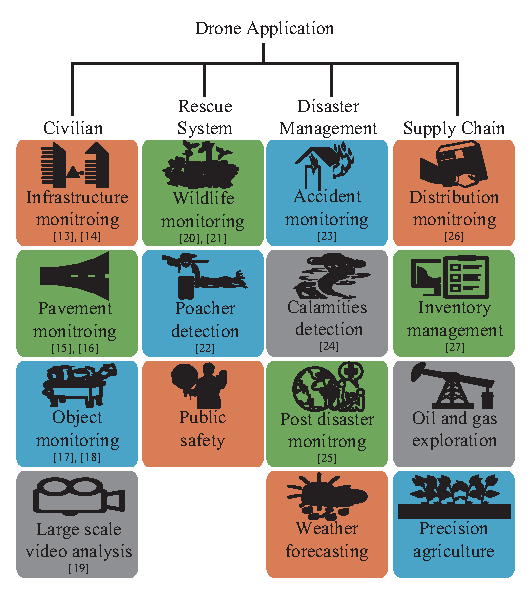
\includegraphics{figure/applicaitonfig.eps}
% \caption{Evaluation of commercial drone usage.}
% \label{applicaitonfig}
% \end{figure}